\section{Stack of Tasks}

'Stack of Tasks' is a hierarchical jacobian-based task controller framework which implements the generalized inverse kinematic formalism by Hanafusa et Al. for local control of redundant systems\cite{hanafusa1981analysis}\cite{Mansard2009ik}. The framework in the earlier stages implemented the Siciliano's extension to handle multiple equality tasks\cite{siciliano1991general}. It has evolved to handle inequality constraints implementing the state of the art solver. The framework provides a structure that orders actives tasks to compute the control law without compromising on the task priority and control continuity. The framework provides a simple scripting interface to interact with controller components during the runtime and has a wrapper to communicate with the ROS world.
\subsection{State of the Art}
Since a 6-axis robot was designed at Stanford allowing a systematic way to design a robot and compute inverse kinematic solution analytically in the seventies, robots have been widely used for a variety of applications from punching cards and palletizing food items to assembly , welding in big automobile manufacturing lines and intelligent stock handling in warehouses \cite{scheinman1969design}. Safety and reliability became a significantly potential area of research since then \cite{dhillon2012robot}. These robots are usually installed in closed chambers, fixed on the ground and absolute care is taken not to make it operational when the door is open or when the co-worker is around the robot’s workspace {safetyreqs}. The safety guidelines are obviously strict as it is crucial to avoid humans in danger. But things are changing quite rapidly and we have an increased focus on human-robot collaboration with enhanced safety in the last decade \cite{Bicchi2008,dhillon2012robot} driven by creative industrial demands and high interest in flexible mobile manipulators. The safety is evaluated based on various factors influencing the human-robot collision impact such as the proximity distance, relative velocity, robot inertia and so on \cite{Kulic2006}. One of the main requirement is the robot’s capability to perceive the environment and react to it.



%    \begin{figure}[thpb]
%       \centering
%       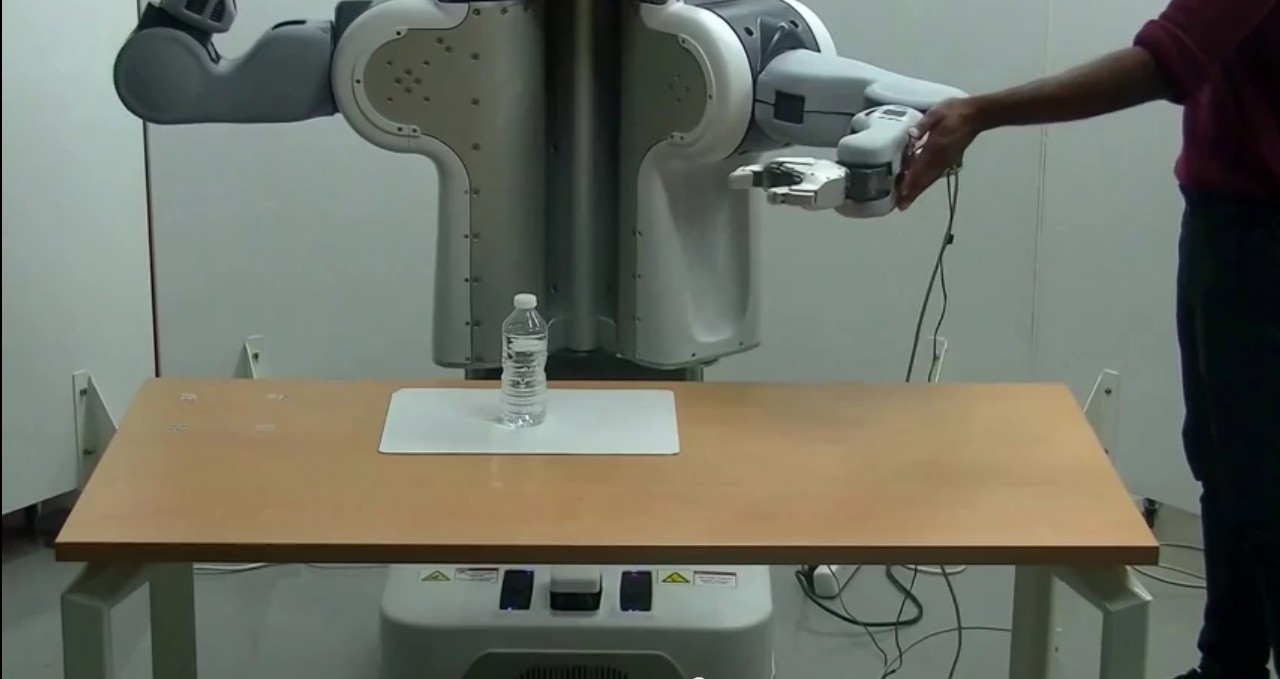
\includegraphics[scale=0.2]{doa/images/skin.eps}
%       \caption{A mobile manipulator executing a trajectory to reach a pre-grasp pose while the forearm is approached by a person with his hand. A skin sensor mounted on the forearm is used to sense any obstacle in the proximity. }
%       \label{figurelabel}
%    \end{figure}

Collision avoidance is an essential functionality in terms of safety and it is a well researched topic with various approaches  to handle different scenarios. In the earlier times, the approaches model the obstacles as static entities treating them as a planning problem to avoid collisions \cite{van2011reciprocal}. Replanning is performed based on instantaneous observations if the obstacles are dynamic. These planning based approaches limit the low level control to simple operations with controller frequencies  several times smaller than robot-environment iteration time. Constrained based approaches focus on enhancing low level control to perform complex operations by taking sensor data directly to be reactive enough with the environment \cite{khatib1986real}. The Collision avoidance can be modeled as inequality constraints or tasks in an optimization based controller. There are a variety of possible inequalities both in robot and environment in robot application scenarios. Some examples are joint limits, singularity avoidance, and object tracking in visual servoing. Constraint based robot programming were used extensively to resolve these constraints  locally but were specific to robot and the scenario involved.

Morover  redundant systems are popular due to their increased flexibility of arm and a mobile base to handle inequality constraints. The control of redundant robots is not trivial as it is not always easy to compute  analytic inverse kinematic and dynamic solutions. Task function based approach  resolves redundancy to minimize the error in task space \cite{Samson1991}. They are jacobian based techniques inverting the differential mapping that maps the control space and the error space to compute optimal controller outputs. A systematic framework for redundant system control proposed by Siciliano allowed to execute multiple tasks simultaneously with priorities {siciliano1991general}. These framework can only solve equality tasks and various strategies focuses on transforming inequality constraints to equalities\cite{Nelson95strategiesfor,chan1995weighted,mansard2009directional,raunhardt2007progressive}. These strategies are not generic enough and has priority inversion problems making them unreliable for practical use. 

A cascade approach was alternatively used to represent the inequalities and equalities systematically as a hierarchical least square program[Kanoun 2011] but suffered from computational inefficiencies. Hierarchical quadratic program (HQP) solver uses complete orthogonal decomposition (COD) instead of singular value decomposition (SVD) and an improved search algorithm which makes it more efficient than available solvers \cite{escande2014hierarchical}. Though constraint based approaches are quite an efficient way to handle collisions and a flexibile way to model them, the are merely locally optimal controllers and does not provide a systematic way to escape local minima. This necessitates the support of global path planners to find the optimal path for realizing a robot task. Combining global path planning and a reliable reactive control is an essential need for deploying robots from simple to complex scenarios.

 
\subsection{What is a Task?}
A task basically composes a control law with a specific objective which can be such as reaching a desired joint position, avoiding obstacles in the environment, a visual servoing mechanism for grasping or so on. A task is mainly defined by the error between the desired and current feature, the error jacobian and the gain. These defined tasks are pushed into 'Stack of Tasks' which computes the control law for all the task objectives in an iterative manner\cite{mansard2007task}. 

\[\textit{e(t) = x\textsuperscript{*} - x }\]

where \textit{x} refers to the current state of a feature, \textit{x\textsuperscript{*}} refers to the reference feature.

\subsection{Redundancy Formalism}
Siciliano and Slotine proposed a systematic control framework to compute controller outputs for achieving multiple tasks in redundant systems from the redundancy formalism proposed by Hanafusa et al. The idea is, tasks are solved only in the null space of the higher priority tasks to avoid conflicts with them. This means, a task at any level has no effect on the tasks in the higher level as it uses only the left degrees of freedom. 

Let $(e_{1},J_{1})$ be a primary task  which is defined by  
\begin{equation} \label{eq:tf1}
\dot{e} = J\dot{q} 
\end{equation}
 \textit{J} referring to the Jacobian of the error velocity with respect to joint velocity at the current joint state.


\begin{equation} \label{eq:tf3}
\dot{q} = J_{1}^{+}\dot{e}_{1} + Pz
\end{equation}
 Where \textit{P} is the projector on the null space of the the Jacobian J and \textit{ $z$ } is the arbitrary velocity vector which can be used as a parameter to achieve the secondary objectives. 

Let $(e_{1},J_{1})(e_{2},J_{2})...(e_{n},J_{n})$ be tasks in the stack. The redundancy formalism for two tasks can be extended to n tasks such that $e_{i}$ does not conflict with $e_{j}$ such that $j<i$. 


The recursive joint velocity is of the form
\begin{equation} \label{eq:ntasks}
  \dot{q}_{0} = 0\\
\end{equation}
\begin{equation}
  \dot{q}_{i} = \dot{q}_{i-1}+ (J_{i}P^{A}_{i-1})^{+}(\dot{e}_{i} - J_{i}\dot{q}_{i-1}), i= 1..n
\end{equation}



 where $P^{A}_{i-1}$ is the projector onto the null space of the augmented Jacobian $J_i^A = (J_1...J_i)$ and $\widetilde{J}_i = J_iP_{i-1}^A$ is the limited jacobian of the task. The joint velocity achieving all the task objectives is $\dot{q} = \dot{q}_n$. The recursive projector is computed by 
 
 \[P^A_i = P^A_{i-1} - (J_iP_{i-1}^A)^+J^A_{i-1}  \] 
 
 This systematic way of prioritizing tasks allows simultaneous execution of multiple tasks without conflicting each other.
 \subsection{Hierarchical Quadratic Programming}
Mansard et al. proposed an improved QP solver to manage multiple equality and inequality problems in a prioritized hierarchy to handle redundancies[15]. The solver handles equality tasks quite the same like in Siciliano's framework but the solver uses complete orthogonal decomposition(COD) instead of Sing for solving the least squares which is quite faster and efficient. The Hierarchical complete orthogonal decomposition(HCOD), a COD of the jacobian mapping for all the levels is used to compute primal optimum for all the constraints at once making it computationally faster. 

Kanoun et al. and De lasa et. al used a primal active search algorithm which is very expensive due to inefficient optimal active set search involving inappropriate activation and deactivation of constraints at each level along the cascade\cite{de2010feature}\cite{kanoun2011kinematic}. The HQP solver depends on a modified primal active search algorithm to make the optimal active set computation much more efficient. Lexicographic optimization formalism is introduced to maintain the active set at each iteration consistent with prior levels completely eliminating unnecessary constraint deactivations and activations. The solver is ten times faster than the classical solvers and can consider inequalities at any levels of the
hierarchy \cite{escande2014hierarchical}.
\subsection{Proximity Distance Gradient for Collision Avoidance}
The computation of the gradient of the proximity distance between the collision bodies inspired from \cite{lefebvre2005fast} is required to define inequality constraints in Stack of Tasks to avoid self-collision and with external obstacles using a proximity sensor. Let $d$ be the distance between approximated collision bodies $O_1(q)$ and $O_2(q)$. The distance between these bodies and its variation is mapped to joint actuations $q$. The distance gradient can be computed by:
\[ \frac{\partial d}{\partial q} = n_d^{'}(\frac{\partial o_1(q)}{\partial q}- \frac{\partial o_2(q)}{\partial q}) \]

where $n_d^{'}$ is the unit normal distance vector while $o_1(q)$ and $o_2(q)$ are the respective closest points. The gradient of the closest point $p$ of fixed coordinates $(\rho_1(q),\rho_2(q)....\rho_l(q))$ in the local reference frame $(e_1(q),e_2(q)...,e_l(q))$ of a collision object at joint configuration $q$ is

\[\frac{\partial p}{\partial q} =  \sum_{l=1}^{d}\rho_l(q)\frac{\partial e_l(q) }{\partial q}\]

In a 3 dimensional workspace, the expression can be written as 

\[ \frac{\partial p}{\partial q} =  (x y  z)J_\omega + J_\nu \]

where $J_\omega$ is the jacobian of the rotational degrees of freedom $J_\nu$ is the jacobian of the linear degrees of freedom. In case of the external objects, the second part of the equation can be eliminated if the object is static. 

% This work is a direct application of the HQP solver and a first attempt to combine path planning and reactive control in a jacobian based solver framework eliminating a cumbersome architecture handling the information flow between control and planning components. Stack of Tasks, a controller framework that implements the latest HQP solver is used in this work to apply the proposed methodology. The proposed methodology is tested on PR2, a mobile manipulation platform with a skin sensor mounted on the forearm of the robot to demonstrate the collision avoidance while executing a planned trajectory without compromising the final goal of the scenario. 


% The paper is organised as follows. Section \ref{sec:application} describes the solution for dynamic obstacle avoidance and Section \ref{sec:skin} discusses the proximity-sensing robot skin. In Section \ref{sec:sot} the robot motion control architecture to incorporate the collision information as safety
% constraints to dynamically adapt the trajectory is presented. Section \ref{sec:prelim_results}
% presents the preliminary results obtained in two different robot setups. Finally, in Section \ref{sec:conclusions} we present our concluding remarks and a discussion of the current work in progress.
\paragraph{Combining Path Planning and Reactive Motion Control}
The methodology is based on defining the main goal as a workspace constraint and prioritizing between safety tasks and trajectory execution task (in joint space). The figure \ref{gso} gives an intuitive idea about the stack priority order .
   \begin{figure}[thpb]
      \centering
      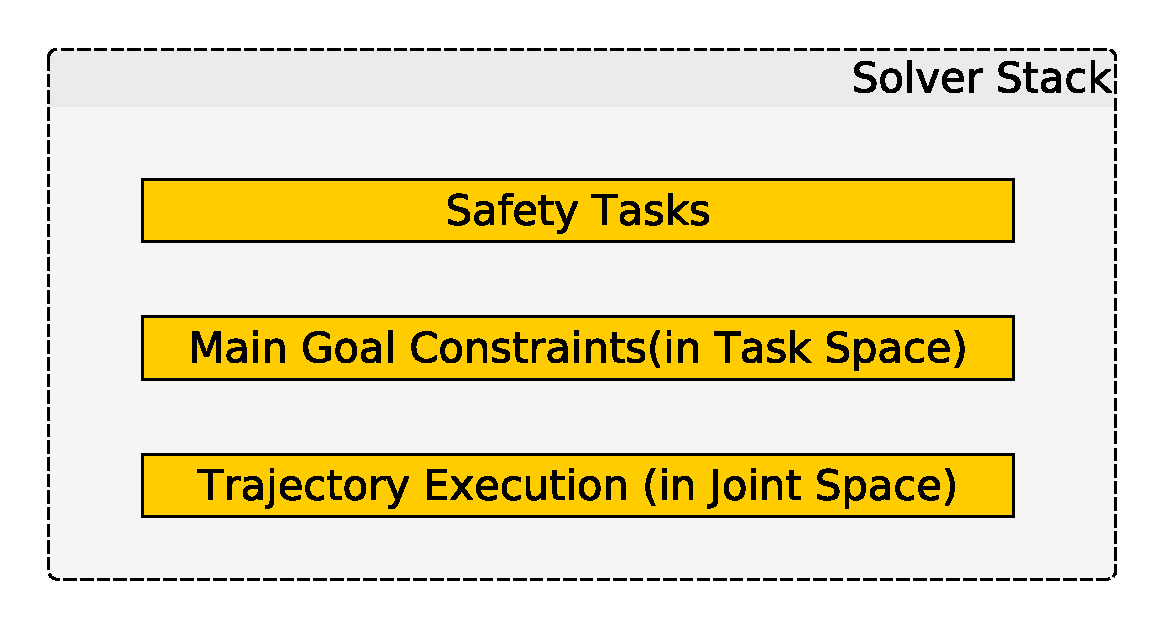
\includegraphics[scale=0.5]{doa/images/ProposedMethodology.eps}
      \caption{Generic stack order for combining planning and control. The priorities decreases from top to bottom. }
      \label{gso}
   \end{figure}

Safety tasks are obviously given higher priority in the stack for collision avoidance. Trajectory execution in Joint space occupies the least priority which leaves the controller only the left degrees of freedom from the primary task. If a base trajectory crosses an unforeseen or dynamic obstacle and if the sensors can sense it, the robot basically cannot execute the trajectory until the object is actually moved out of its way. Replanning could be activated if there is no other possibility to reach the joint trajectory goal. Even if there is a possibility to avoid the obstacle and continue executing the  trajectory, it is always not sure that the robot will end up in the desired goal in the task space. The clever trick here is in the way the main goals are defined. The main goal can be moving a base to a particular pose in the world or move the end effector to a grasping pose. Here the important thing is that the goals are something defined in the workspace though a joint trajectory is executed to achieve them. The hierarchical nature of the controller puts this main goal task in high priority and the jacobian core of the solver finds an optimal solution to follow the main goal. The next section illustrates this methodology on a simple scenario to show the potential of this method.

